\documentclass[11pt, a4paper,twocolumn]{article}
\usepackage[utf8]{inputenc}
\usepackage[left=2cm, text={16cm, 24cm}, top=3cm]{geometry}
\usepackage[czech]{babel}
\usepackage{times}
\usepackage[unicode]{hyperref}
\usepackage{graphicx}

\title{ISS riesenie}
\author{xskuta04}
\date{December 2018}

\begin{document}
\begin{titlepage}

\thispagestyle{empty}
\begin{center}
\Huge
\textsc{Vysoké učení technické v Brně}\hspace{0.4em}\\
\huge{\textsc{Fakulta informačních technologií}}\\
{\includegraphics[width=0.75\linewidth]{include/vut_fit_logo.png}} \\
\hspace{0.4em}\\


\vspace{\stretch{0.382}}
\LARGE{ Signály a systémy \hspace{0.3em}}\\
\Huge {Projekt}\hspace{0.3em}\\
\vspace{\stretch{0.618}}
\end{center}
\Large{15. December 2018 \hfill
xskuta04@stud.fit.vutbr.cz \\
\null \hfill Matúš Škuta(xskuta04)}
\end{titlepage}

\section*{Riešenie}

Zadanie je riešené v programe \texttt{OCTAVE}. Všetky výpočty sa nachádzajú v odovzdanom súbore \texttt{xskuta04.m}. Protokol bol písaný v \LaTeX e.

\begin{enumerate}
    \item
    {
        Vzorkovacia frekvencia signálu je \textbf{16 000 [Hz]}. Dĺžka signálu vo vzorkách je \textbf{32 000}, v sekundách \textbf{2 [s]}. Zvuk som načítal cez funkciu \texttt{audioread}.
    }

    \item
    {
        Prvých 20ms signálu, som dekódoval do binárnych symbolov ktoré sú zobrazené v grafe červenou a modrou je zobrazený signál.
        \begin{center}
        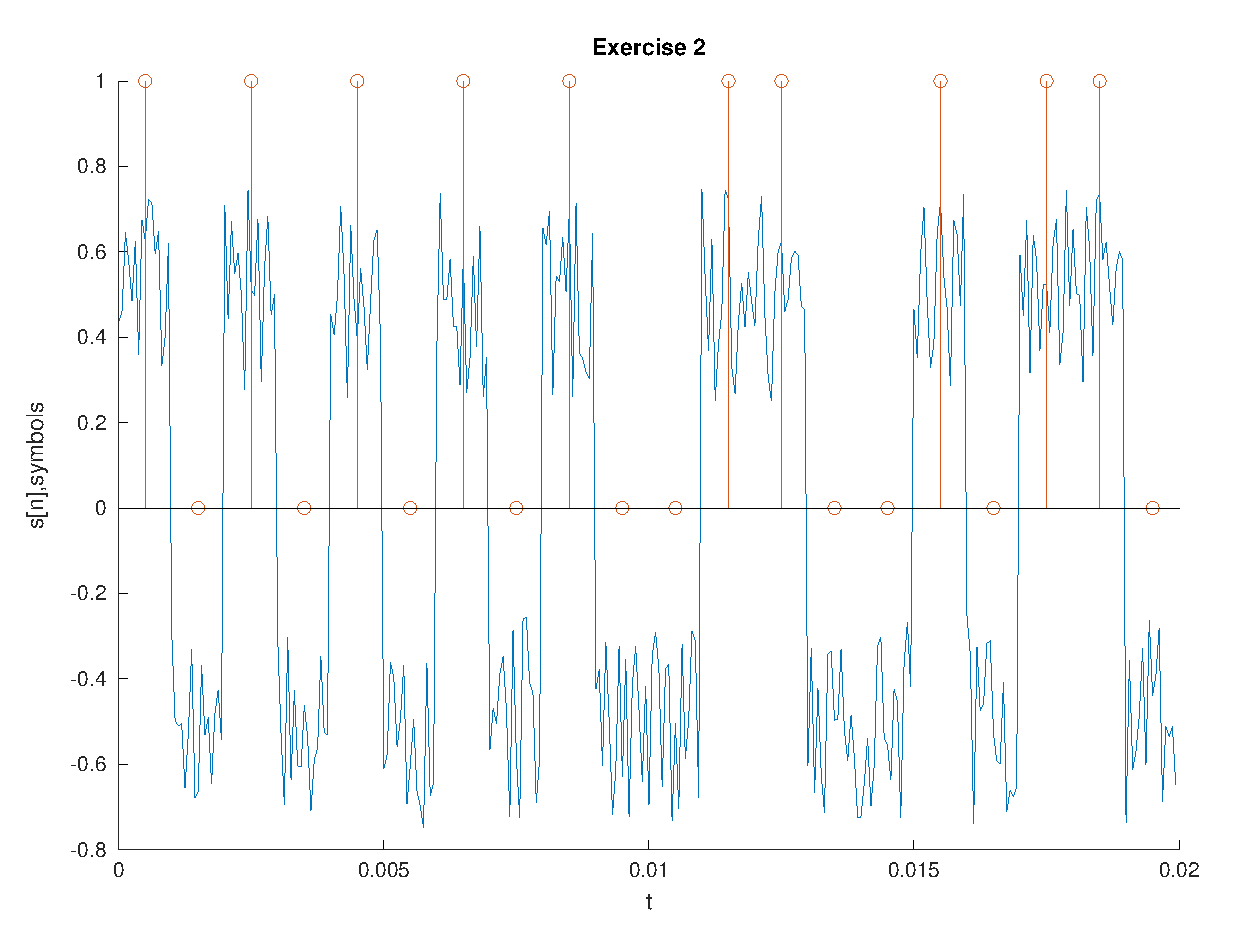
\includegraphics[width=\linewidth,keepaspectratio]{include/2.eps}
        \end{center}
    }

    \item
    {
        \textbf{Filter je stabilný}, pretože pre všetky póly \texttt{$p_k$} platí vzťah \texttt{$|p_k| < 1$}, čo značí že sa nachádzajú vo vnútri kružnice. Obrázok s nulami a pólmi som vytvoril pomocou funkcie \texttt{zplane}.
        \begin{center}
        \includegraphics[width=\linewidth,keepaspectratio]{include/3.eps}
        \end{center}
    }

    \item
    {
        Filter je typu \textbf{dolná priepusť}. Modul kmitočtovej charakteristiky som vypočítal cez funkciu \texttt{freqz} s počtom bodov pre zobrazenie 500. Meznú frequenciu som našiel pomocou funkcie \texttt{min}, ktorá vrátila index ktorý som potom použil pre os \textbf{x}, ktorá mi vrátila hodnotu \textbf{480}.
        \begin{center}
        \includegraphics[width=\linewidth,keepaspectratio]{include/4.eps}
        \end{center}
    }

    \item
    {
        Na filtrovanie signálu bola použitá funkcia \texttt{filter}. Signál som vždy posunul o jedno doľava, vykreslil a porovnal pokial som nenašiel podobu. Výsledok vyšiel posun \textbf{vľavo} o \textbf{16} vzorkov (\textbf{predbehnutie}). Z obrázku je možné vidieť že posun 16 vzorkov do ľava je pravdepodobne dobrý.
        \begin{center}
        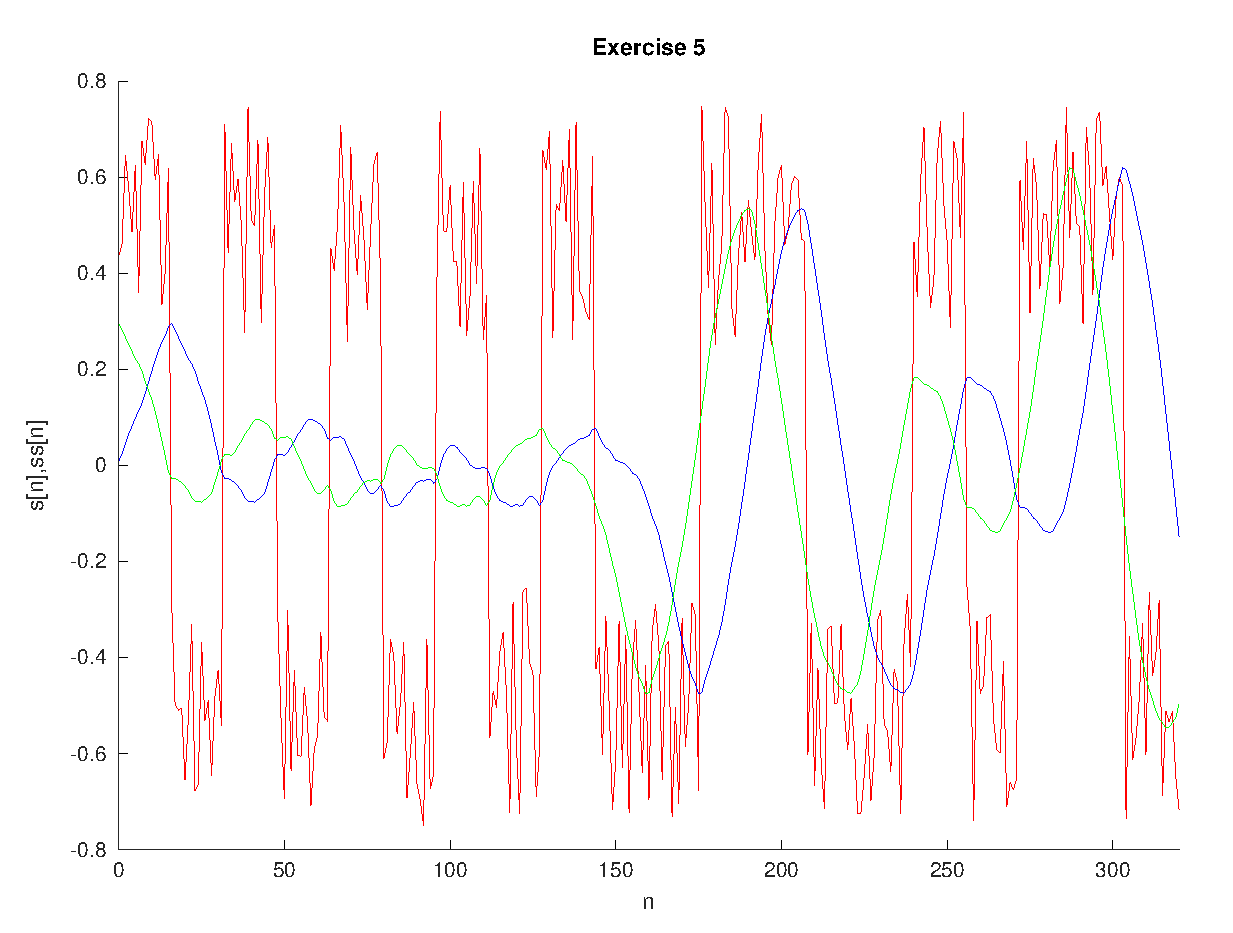
\includegraphics[width=\linewidth,keepaspectratio]{include/5.eps}
        \end{center}
    }

    \item
    {
        Signály som vykreslil pomocou \texttt{plot} funkcie, a binárne hodnoty pomocou \texttt{stem} funkcie.
        \begin{center}
        \includegraphics[width=\linewidth,keepaspectratio]{include/6.eps}
        \end{center}
    }

    \item
    {
        Nakoľko som posúval signál o 16 vzorkov tak som porovnával len 1999 binárnych signálov. Chybovosť signálu vyšla \textbf{5.902951 \%}.
    }

    \item
    {
        Signál som filtroval cez funkciu \texttt{filter} a funkciu \texttt{fft} som použil na spočítanie spektra signálu diskrétnej \textbf{Fourierovej tranformácie}. Pri oranžovom vyfiltrovanom signále si možme všimnúť že po \textbf{480 [Hz]} začne filter potlačovať vysoké frequencie, čo sa zobrazí do Fourierovej tranformácie.
        \begin{center}
        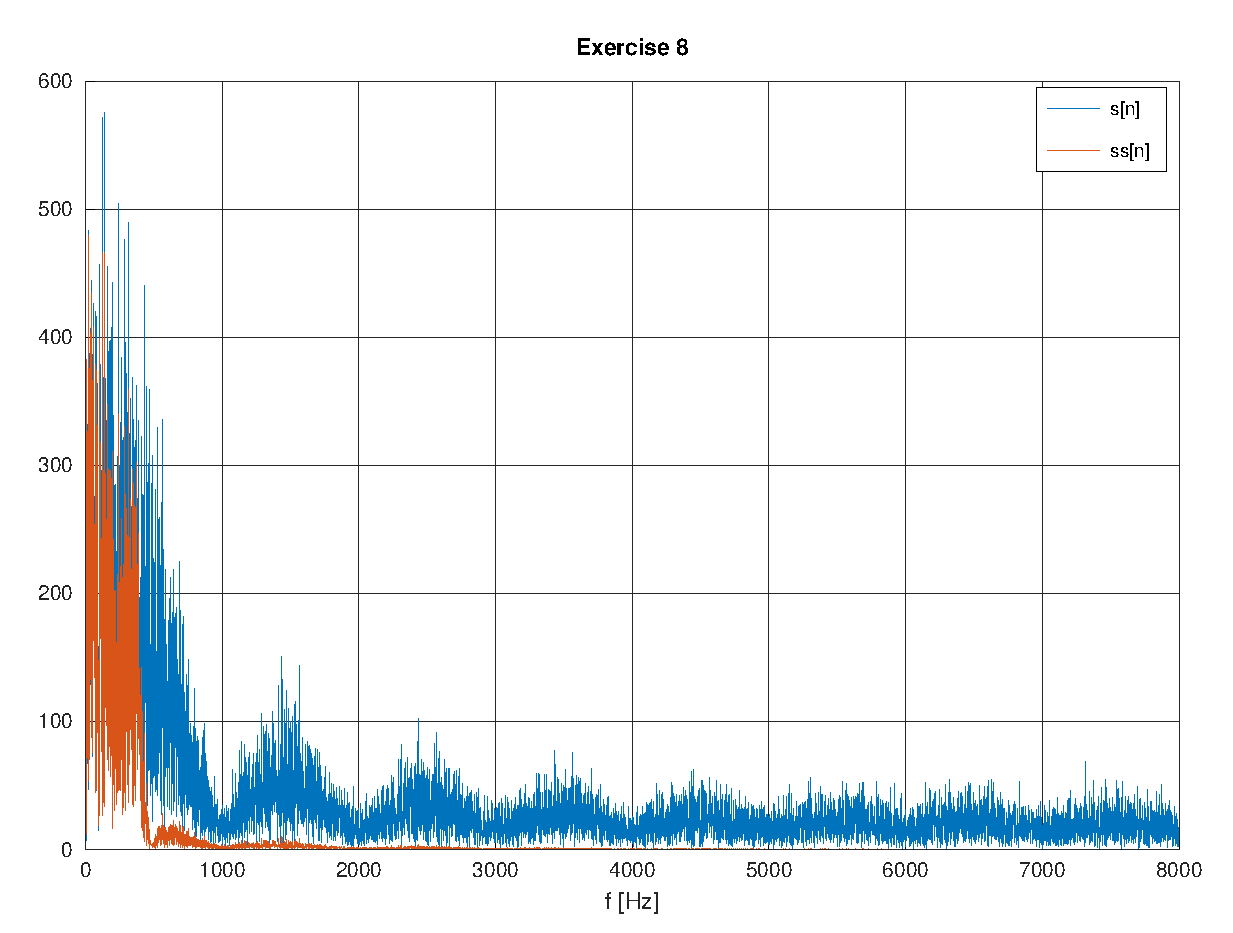
\includegraphics[width=\linewidth,keepaspectratio]{include/8.eps}
        \end{center}
    }

    \item
    {
        Odhad funkcie hustoty môžme vidiet na obrázku, a overenie integrálom platí. $$\int_{x}p(x)dx = 1$$
        \begin{center}
        \includegraphics[width=\linewidth,keepaspectratio]{include/9.eps}
        \end{center}
    }

    \item
    {
        Autokorelačné koeficienty som počítal cez zadanú funkciu \texttt{xcorr}. Vrátený výsledok som vydelil počtom vzorkov originálneho signálu, aby to odpovedalo vzorcu $ R[k] = \frac{1}{N} \sum\limits_n x[n] x[n+k] $.
        \includegraphics[width=\linewidth,keepaspectratio]{include/10.eps}
    }

    \item
    {
        Hodnota koeficientu $R[0]$ : $0.234468$\\
        Hodnota koeficientu $R[1]$ : $0.271120$\\
        Hodnota koeficientu $R[16]$ : $0.000269$
    }

    \item
    {
        Využil som funkciu \texttt{hist2}. Do ktorej som vložil originálny signál spolu s posunutým signálom o 1 vzorok a lineárne rozložený vektor o 50 vzorkoch od najmenšej hodnoty signálu po najväčšiu. Na vykreslenie som využil funkciu \texttt{imagesc}.
        \begin{center}
        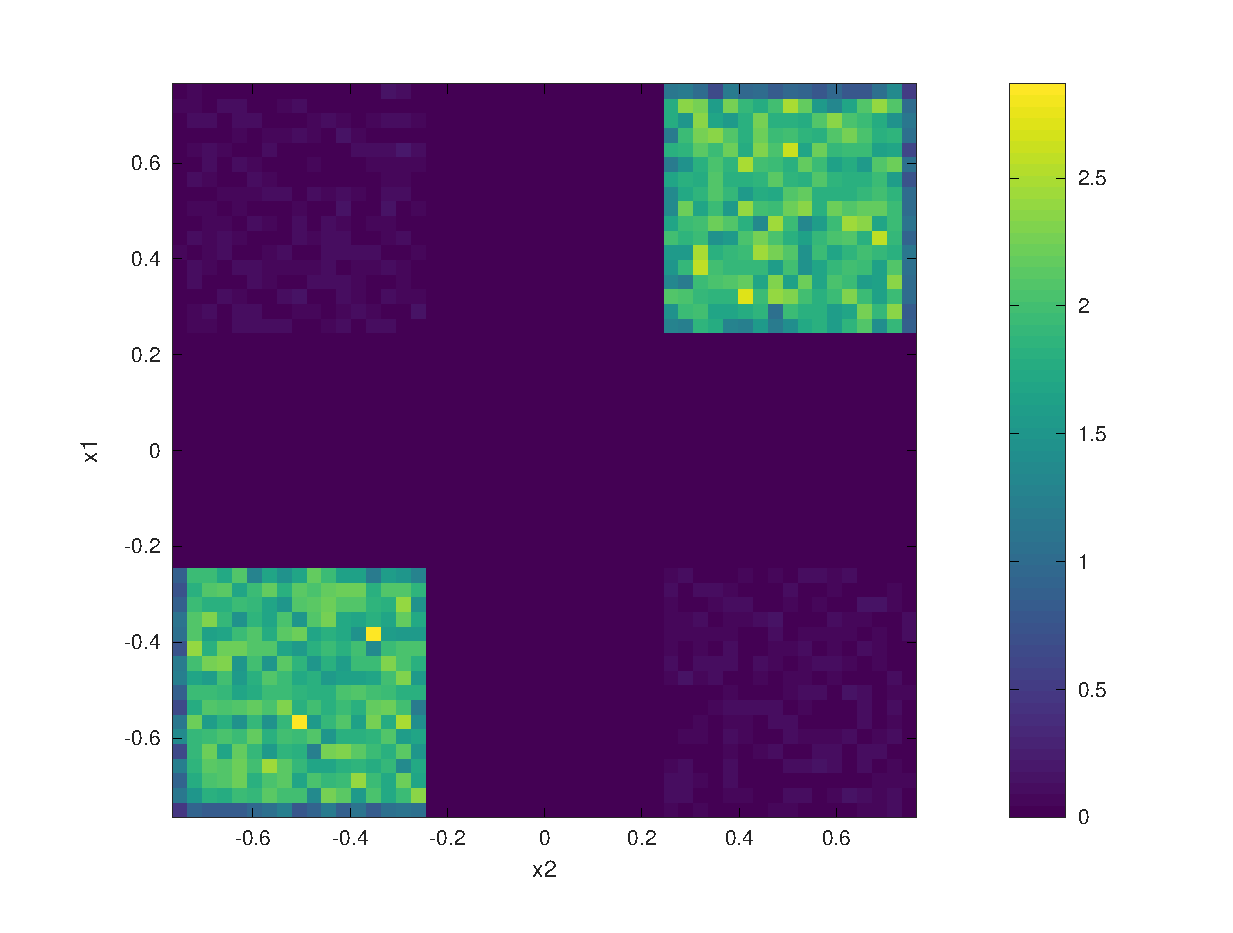
\includegraphics[width=\linewidth,keepaspectratio]{include/12.eps}
        \end{center}
    }

    \item
    {
        Funkcia \texttt{hist2} za mňa otestovala $$ \int_{x_1} \int_{x_2} p(x_1,x_2,1)dx_1dx_2 = 1$$ a vyšlo že sa rovná \textbf{1}.
    }

    \item
    {
        Na vypočítanie korelačného koeficientu som využil časť funkcie \texttt{hist2}, jej výsledok bol \textbf{0.234581}. Výsledok mal z hodnotou koeficientu \textbf{R[1]} z 11 úlohy podobnosť iba pri 3 desatinných miestach, lebo sa jedná o iteračný spôsob výpočtu ktorý je menej presný.

    }
\end{enumerate}

\end{document}
